\chapter{Application Architecture}\label{chapter:application_architecture}
\todoin{Next few pages should describe the architecture of your solution including UML diagrams, interaction with other systems and dependencies on external libraries}
The \gnb{} application was built using a PHP backend and a web-based (HTML + Javascript) frontend. Also, the solution may provide the clients of \gnb{} with an additional SCS (short for Smart-Card-Simulator) software, which is needed to provide 2-step authentication during transactions and can be used on any system that supports Java 1.7+.\newline
The application was almost entirely developed without the aid of external libraries, preferring the use of builtin APIs and a custom architecture. Here is a list of the used libraries, which will be later on described more in details, along with their interaction with the system:
\begin{itemize}
	\item PHPMailer (see \texttt{https://github.com/PHPMailer/PHPMailer})
	\item fpdf (see \texttt{http://www.fpdf.org/})
	\item pdf encryption script using fpdf (see \texttt{http://www.fpdf.org/en/script/script37.php})
	\item secureimage (see \texttt{https://github.com/dapphp/securimage})
\end{itemize}

In the following section we will discuss the architecture of the whole web application; we will also provide dedicated sections for a more detailed analysis of the Entity-Relationship model used in the database as well as the architecture of the Smart Card Simulator.
\section{Architecture}

\section{Database Schema}\label{section:db}
\begin{figure}[h!tbp]
	\centering
	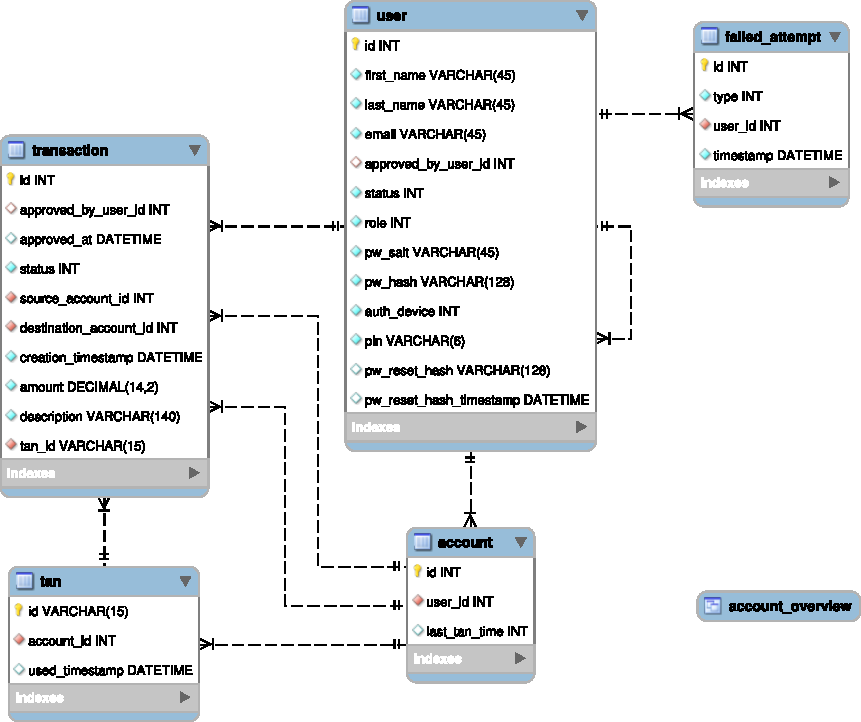
\includegraphics[width=\textwidth]{figures/database_model}
	\caption{Database model}
	\label{figure:dbmodel}
\end{figure}

The database schema was created using the \emph{MySQL Workbench}. The database schema is shown in \autoref{figure:dbmodel} and describes the following 6 entities:
\begin{description}
	\item[Table "user"] \hfill \\
	Contains all the user attributes including user ID, full name, mail, status (\texttt{unapproved}, \texttt{approved}, \texttt{rejected}, \texttt{blocked}), role (\texttt{client}, \texttt{employee}), salt and hash for the authentication, the device used for TAN authentication (\texttt{none} for users without account, otherwise \texttt{TANs} or the \texttt{SCS}), the PIN as well as the password reset hash and creation timestamp for this hash. Additionally the user ID is stored which approved/blocked/rejected the user the last time.
	
	\item[Table "account"] \hfill \\
	Contains the account number, the user ID of the owner and the timestamp of the last TAN that was used if the user is using the SCS (see \autoref{section:scs}).
	
	\item[Table "transaction"] \hfill \\
	Contains information about the status (\texttt{unapproved}, \texttt{approved}, \texttt{rejected}), the user ID of the approving/rejecting user and approval/rejection time of the transactions as well as the source and destination account, creation timestamp, amount and description of the transaction as well as the used TAN (if the SCS was not used).
	
	\item[Table "tan"] \hfill \\
	Contains the TANs and which account they belong to as well as a field specifying if the given TAN has been used (value is a timestamp) or not used (value is \texttt{NULL}).
	
	\item[Table "failed\_attempt"] \hfill \\
	Contains all failed attempts (e.g. failed \texttt{login} or invalid \texttt{tan}) and their timestamp associated to the user ID that attempted the action.
	
	\item[View "account\_overview"] \hfill \\
	Is used to obtain the balance for a given account number. As shown in \autoref{figure:accountoverviewfigure} this approach is not trivial. First (lines 8-9) we set Barney's balance to a fixed amount because all the welcome credits to new users are coming from his account. Then we exclude some transactions from our calculation, namely rejected transactions, unapproved transactions and transactions that have the same source- and destination account number (see lines 12-14). After that we determine the sign of the transaction --- it is either positive if the given account is the destination account, or negative if our account is the source account (see lines 17-19).
	
\begin{figure}[h!tbp]
	\centering
	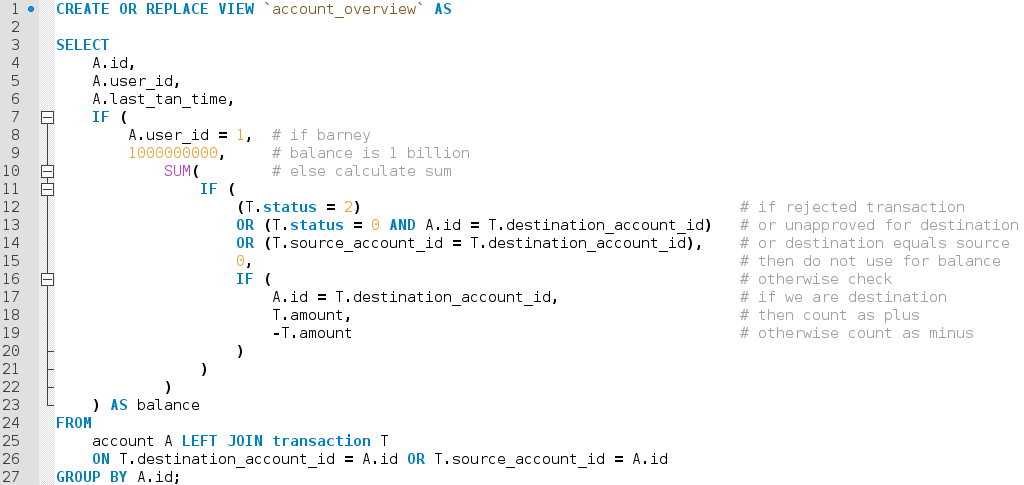
\includegraphics[width=\textwidth]{figures/code_account_overview}
	\caption{View "account\_overview"}
	\label{figure:accountoverviewfigure}
\end{figure}

\end{description}

\section{Smart Card Simulator}\label{section:scs}
